 \taskpic{ Круглое отверстие радиусом $r$ в дне сосуда, первоначально
  заполненном водой, для герметизации закрыто шаром массой $m$ и
  радиусом $R>r$. Уровень воды медленно понижают, и когда он достигает
  некоторого значения $h_0$, шар поднимается над отверстием. Найдите
  $h_0$. }
{
  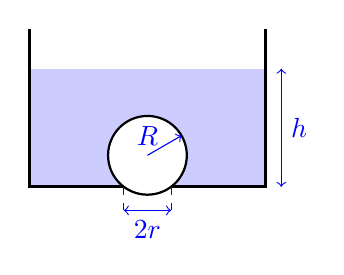
\begin{tikzpicture}
    \draw[fill=blue!20,draw=white] (0.5,0) rectangle (3.5,1.5);
    \draw[very thick] (0.5,2) -- (0.5,0) -- (3.5,0) -- (3.5,2);
    \draw[thick,fill=white] (2,0.4) circle (0.5cm);
    \draw[blue,<->] (3.7,0) -- (3.7,1.5) node[midway,right] {$h$};
    \draw[blue,->] (2,0.4) node[above] {$R$} -- ++(30:0.5);
    \draw[blue,dashed] (1.7,0) -- (1.7,-0.3);
    \draw[blue,dashed] (2.3,0) -- (2.3,-0.3);
    \draw[blue,<->] (1.7,-0.3) -- (2.3,-0.3) node[midway,below] {$2r$};
  \end{tikzpicture}
}